\tikzset{>=latex} % for LaTeX arrow head

% DRAW PLOT: sin, cos, tan


\begin{tikzpicture}[domain=-pi:pi,xscale=2/pi]
%https://tex.stackexchange.com/questions/45151/format-numbers-as-a-fraction-of-pi-with-tikz-pgfmathprintnumber
  
  % limits
  \def\xa{ -pi-0.3}
  \def\xb{3*pi+0.4}
  \def\ya{-3.4}
  \def\yb{ 3.6}
  \def\N{100} % number of points
  
  % axes & grid
  \draw[xstep=pi/2,very thin, color=gray]
    (\xa,\ya) grid (\xb,\yb);
  \draw[->]
    (\xa,0) -- (\xb,0)
    node[right] {$x$};
  \draw[->]
    (0,\ya) -- (0,\yb)
    node[left] {$y$};
  
  % ticks
  \draw[] % x
  	node[below,scale=0.9] at ( -pi,   0) {$-\pi$}
  	node[below,scale=0.9] at ( -pi/2, 0) {$-\dfrac{\pi}{2}$}
  	node[below,scale=0.9] at (     0, 0) {0}
  	node[below,scale=0.9] at (  pi/2, 0) {$\dfrac{\pi}{2}$}
  	node[below,scale=0.9] at (  pi,   0) {$\pi$}
  	node[below,scale=0.9] at (3*pi/2, 0) {$\dfrac{3\pi}{2}$}
  	node[below,scale=0.9] at (2*pi,   0) {$2\pi$}
  	node[below,scale=0.9] at (5*pi/2, 0) {$\dfrac{5\pi}{2}$}
  	node[below,scale=0.9] at (3*pi,   0) {$3\pi$};
  \draw[] % y
  	node[left,scale=0.9] at ( 0,  3) {$3$}
  	node[left,scale=0.9] at ( 0,  2) {$2$}
  	node[left,scale=0.9] at ( 0,  1) {$1$}
  	node[left,scale=0.9] at ( 0,  0) {$0$}
  	node[left,scale=0.9] at ( 0, -1) {$-1$}
  	node[left,scale=0.9] at ( 0, -2) {$-2$}
  	node[left,scale=0.9] at ( 0, -3) {$-3$};
  
  % functions
  \def\ea{0.28}
  \def\eb{0.26}
  \draw[color=blue,samples=\N,domain=\xa:\xb] % SIN
    plot(\x,{sin(\x r)}) % r for radians
    node[above right] at (5*pi/2,1) {$\sin(x)$};
  \draw[color=red,samples=\N,domain=\xa:\xb] % COS
    plot(\x,{cos(\x r)})
    node[above left] at (2*pi,1) {$\cos(x)$};
  \draw[color=orange] % TAN
    plot[samples=\N,domain=  \xa     :   -pi/2-\eb] (\x, {tan(\x r)})
    plot[samples=\N,domain=  -pi/2+\ea:   pi/2-\eb] (\x, {tan(\x r)})
    plot[samples=\N,domain=   pi/2+\ea: 3*pi/2-\eb] (\x, {tan(\x r)})
    plot[samples=\N,domain= 3*pi/2+\ea: 5*pi/2-\eb] (\x, {tan(\x r)})
    plot[samples=\N,domain= 5*pi/2+\ea:  \xb      ] (\x, {tan(\x r)})
    node[samples=\N,right=-2pt] at (pi/2,2.5) {$\tan(x)$};
  
\end{tikzpicture}
